\chapter{Blockchain Notarization: A Practical Use Case}
\label{chpr:project}
This Chapter is aimed to be a technical report of a project in which the author, in partnership with DGI (Digital Gold Institute) and ANIA (Associazione Nazionale fra le Imprese Assicuratrici), worked during the draft of this thesis.

\bigskip
\section{Executive Summary}
The purpose of this project work is to provide future clients a fully operating timestamping service, to enforce the notarization of digital documents which, as we already know, is traditionally achieved by certification authorities (CA), with a decentralized solution that is resilient even if the security of such CA is violated from the inside.

\bigskip
\noindent
The timestamping service is implemented, with some extensions and modification on the basis of need, according to the \textit{OpenTimestamps} protocol, because of its high scalability and low maintenance cost, all nice features that we already saw in the description of such protocol in Section \ref{sec:ots}. In addition, the proposed solution is independent of any provider, being \textit{OpenTimestamps} an open-source project. It could be made available to customers for free or in form of a subscription service, with specific service level agreements, in order to provide additional features like the custody of any user's timestamp proof. For example, any insurance company could make use of this solution to grant authenticity of its associates' insurance policies or, more generally, whenever a digital signature is involved. We remind that \textit{OpenTimestamps} also provides all the guarantees for an independent audit: a user can verify the validity of its timestamp proof without the need of the calendar server which actually maintains the service up, just by querying a local Bitcoin node or a public block explorer. Next we will move on the technical details regarding how this service is built, specifying when the \textit{OpenTimestamps} protocol is improved.

\bigskip
\section{Architecture of the Solution}
The architecture of the solution is composed by three servers (in cloud), accessible from outside via https thanks to network components.

\bigskip
\noindent
A user can easily connect to the public web server via browser at \url{https://timestamp.aniasafe.it} and drag a document to timestamp\footnote{We remind that what is really timestamped is the \textit{hash value} of such document, automatically computed on user's local device, without harming privacy. We refer to Chapter \ref{chpr:notarization} for all the details.}. It is directly from browser (thanks to the underlying JavaScript code) that the timestamp request is sent to the calendar servers to be processed. The corresponding timestamp proof is automatically downloaded on the user's local device and can be verified on the same web page, simply dragging the \colorbox{light-gray}{.ots} file. In that specific case, the browser will query public block explorers\footnote{As specified in Section \ref{sec:ots-web}, timestamping services deployed as browser applications cannot query a local Bitcoin node and have to trust public block explorers.} in order to perform the verification procedure. 

\bigskip
\noindent
Before getting into technical details regarding the code that underlies this solution, we present two explanatory figures. On one hand, Figure \ref{fig:ots-project-stamping} is aimed to give an abstract idea of the whole timestamping process, on the other hand Figure \ref{fig:ots-project-verifying} refers to the verification procedure.

\begin{figure}[ht]
    \centering
	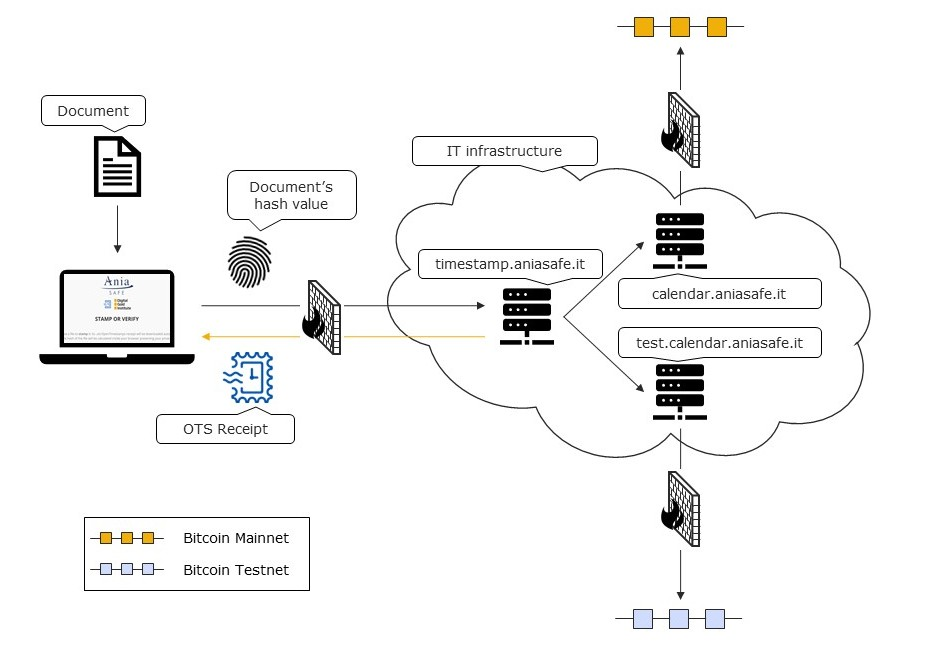
\includegraphics[width=1\linewidth]{Images/project-stamping.jpg}
	\caption{Architecture of the timestamping process}
	\label{fig:ots-project-stamping}
\end{figure}

\bigskip
\begin{figure}[ht]
    \centering
	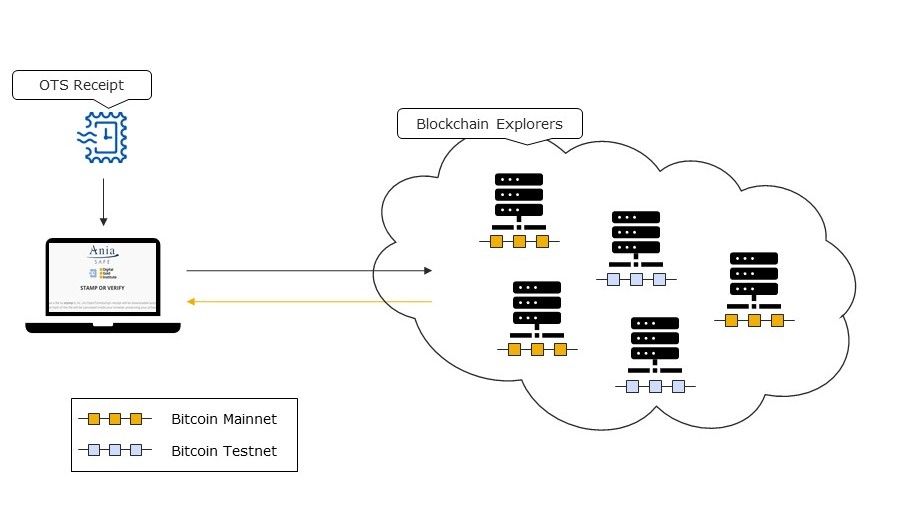
\includegraphics[width=1\linewidth]{Images/project-verifying.jpg}
	\caption{Architecture of the verification process}
	\label{fig:ots-project-verifying}
\end{figure}

\bigskip
\section{Technical Details}
The three servers introduced before are divided in a front-end server (\url{https://timestamp.aniasafe.it}) which hosts the public web page, and two back-end servers, the first one running a calendar server connected to a local\footnote{In the sense that the calendar server and the Bitcoin node run on the same machine.} Bitcoin node in mainnet mode (\url{https://calendar.aniasafe.it}), the latter connected to a local one in testnet mode (\url{https://test-calendar.aniasafe.it}).